
%###############################################################################
\section{排序与查找}
%###############################################################################

%-------------------------------------
\subsection{排序算法}
%-------------------------------------

%-----------------

\begin{frame}[fragile]{7.3.1~排序算法}

排序是数据处理的最基本任务,目的是按照某种规则将一组无序数据重新排列,使之有序。

\vspace{-4mm}
\begin{columns}[t]

\column{0.65\textwidth}
\begin{blueblock}<2->{\texttt{Array}类模板定义四}
\vspace{-3mm}
\begin{lstlisting}[moreemph={Array,T}]
template<typename T, size_t N>
class Array {
public:
    template<typename F = Less<T> >
    void selectionSort(F f = F());      //选择排序
    template<typename F = Less<T> >
    void insertionSort(F f = F());      //插入排序
    template<typename F = Less<T> >
    void bubbleSort(F f = F());         //冒泡排序
private:
    void swap(int i, int j){
        T t = m_ele[i];
        m_ele[i] = m_ele[j];
        m_ele[j] = t;
    }
};
\end{lstlisting}
\vspace{-1mm}
\end{blueblock}

\column{0.3\textwidth}
\begin{yellowblock}<2->{说明}
成员\texttt{swap}函数用来交换两个元素的位置,它仅在\texttt{Array}类内部使用,因此它的访问属性为\texttt{private}
\end{yellowblock}

\end{columns}

\end{frame}

%-----------------

\begin{frame}[fragile]{7.3.1 排序算法\normalsize{~---~选择排序}}

每次在待排序元素中选择最小的一个,换放到已排序数列后面

\vspace{1mm}

\begin{center}
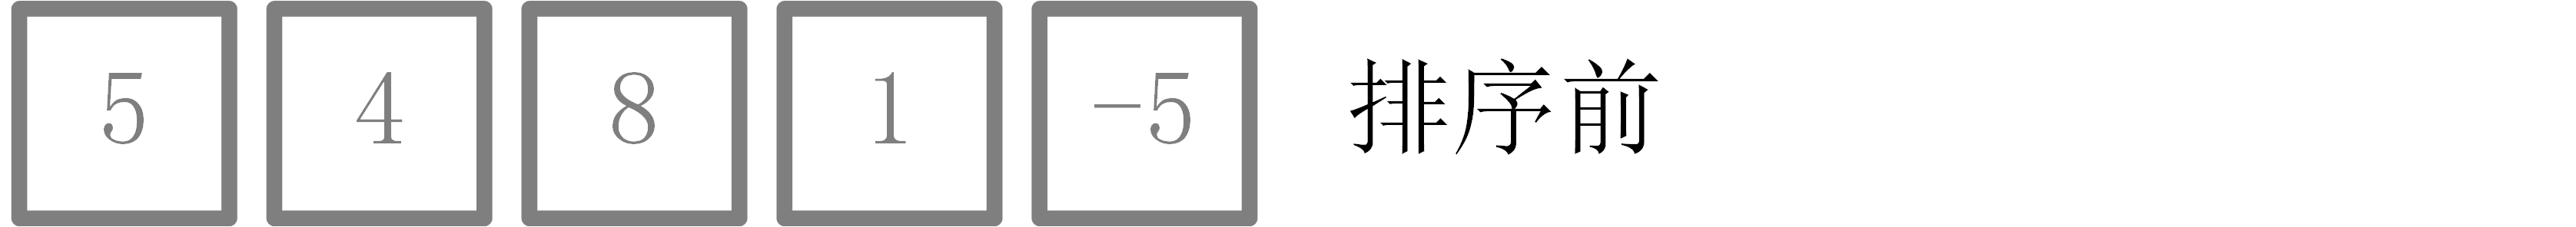
\includegraphics[width=0.8\textwidth]{selection_sort_1}\\\vspace{3mm}
\uncover<2->{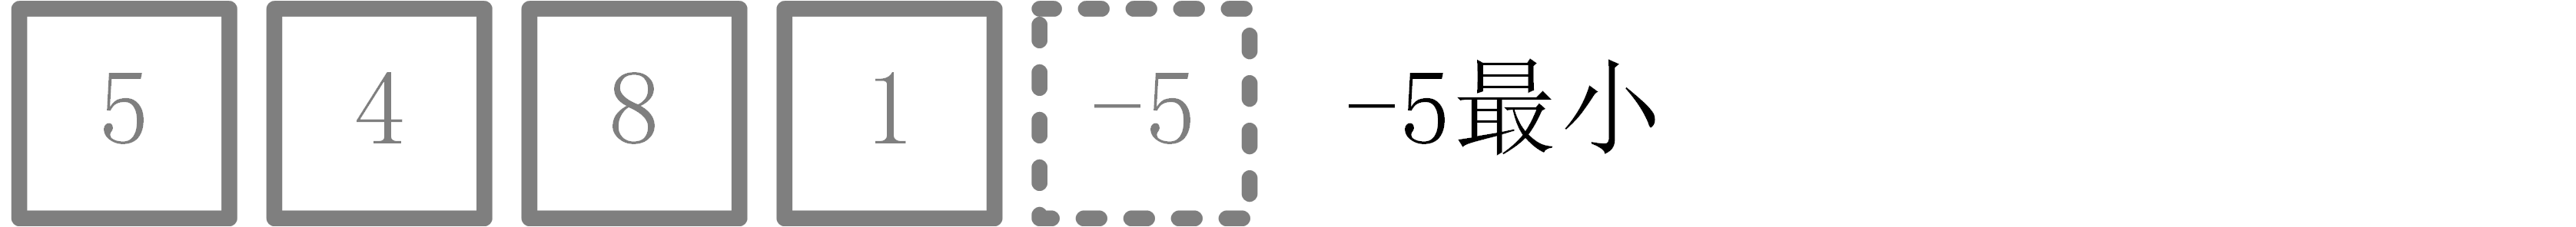
\includegraphics[width=0.8\textwidth]{selection_sort_2}}\\\vspace{-11mm}
\uncover<3->{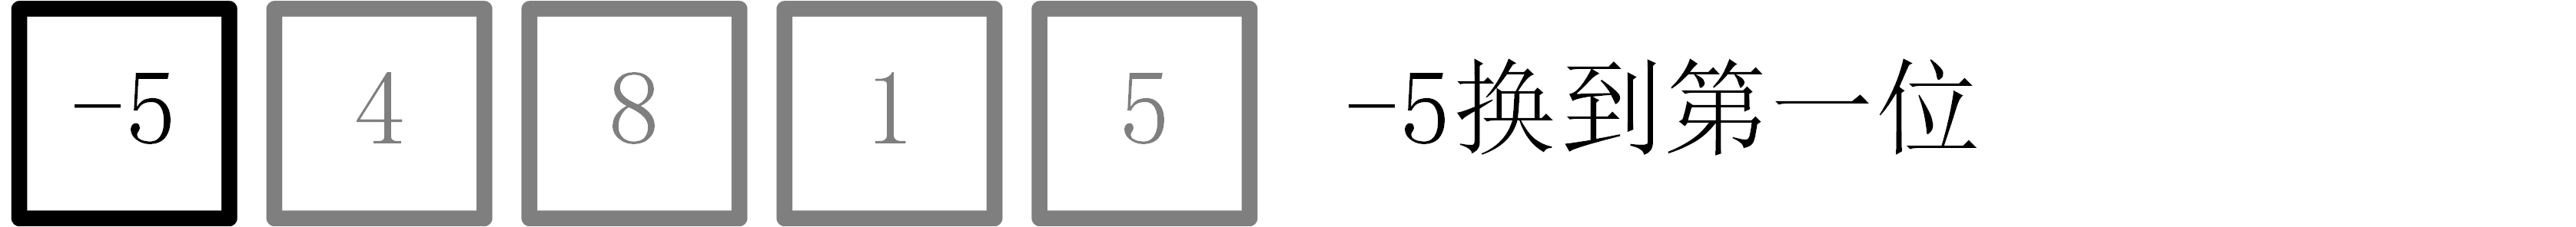
\includegraphics[width=0.8\textwidth]{selection_sort_3}}\\
\uncover<4->{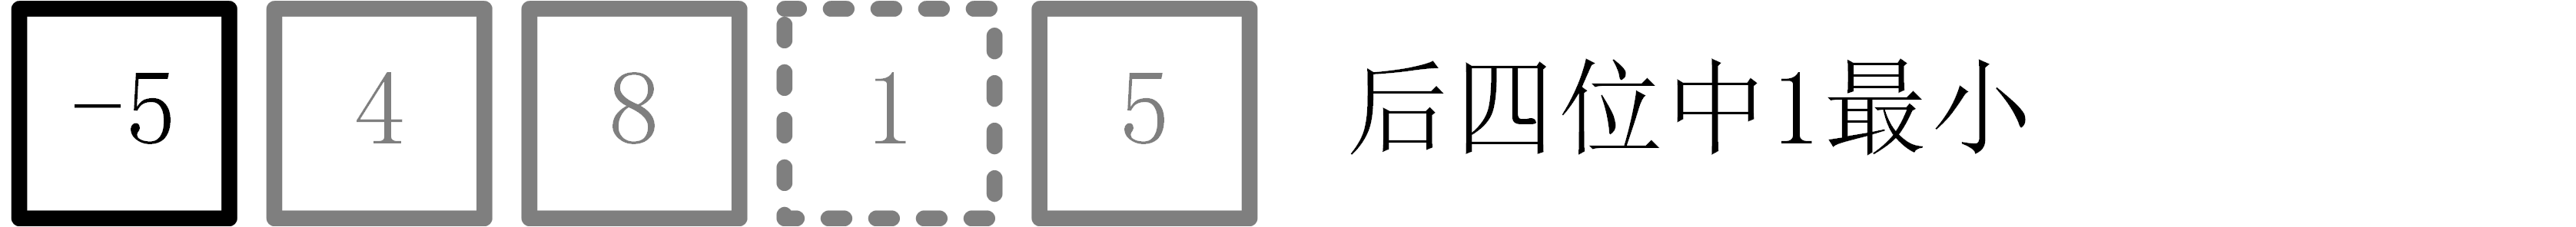
\includegraphics[width=0.8\textwidth]{selection_sort_4}}\\\vspace{-11mm}
\uncover<5->{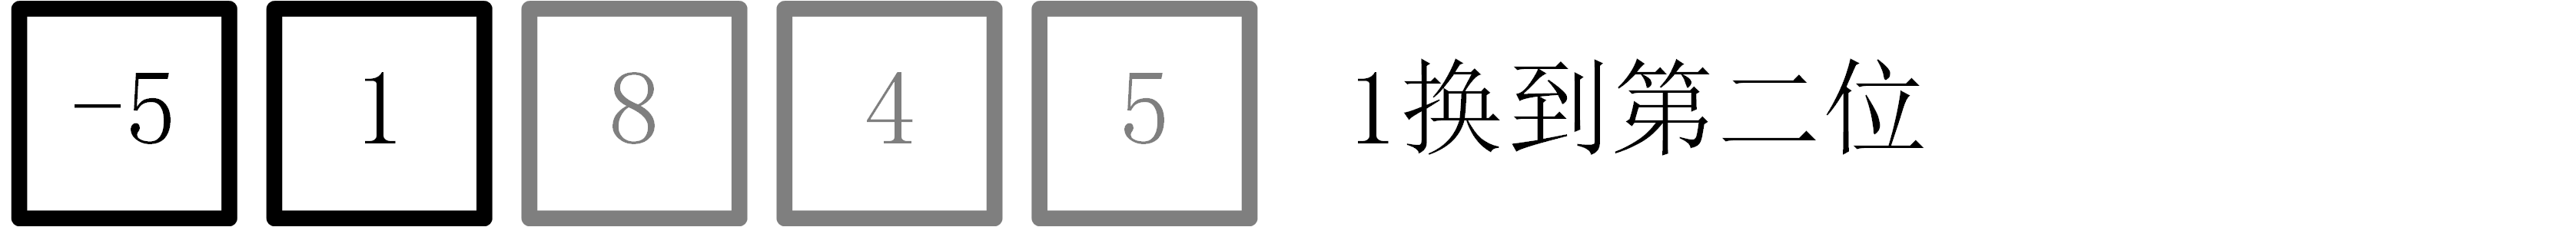
\includegraphics[width=0.8\textwidth]{selection_sort_5}}\\
\uncover<6->{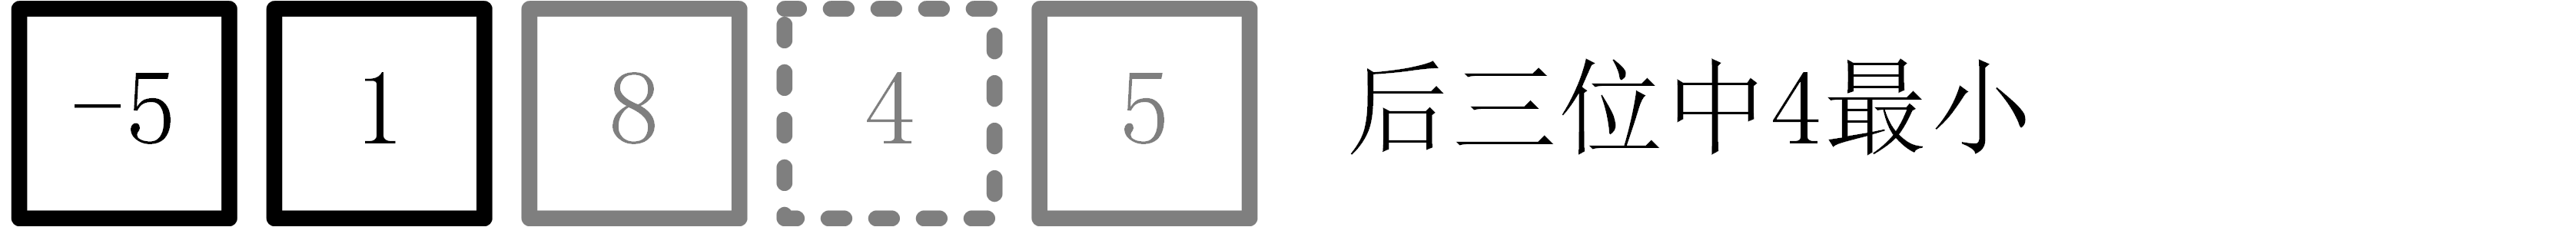
\includegraphics[width=0.8\textwidth]{selection_sort_6}}\\\vspace{-11mm}
\uncover<7->{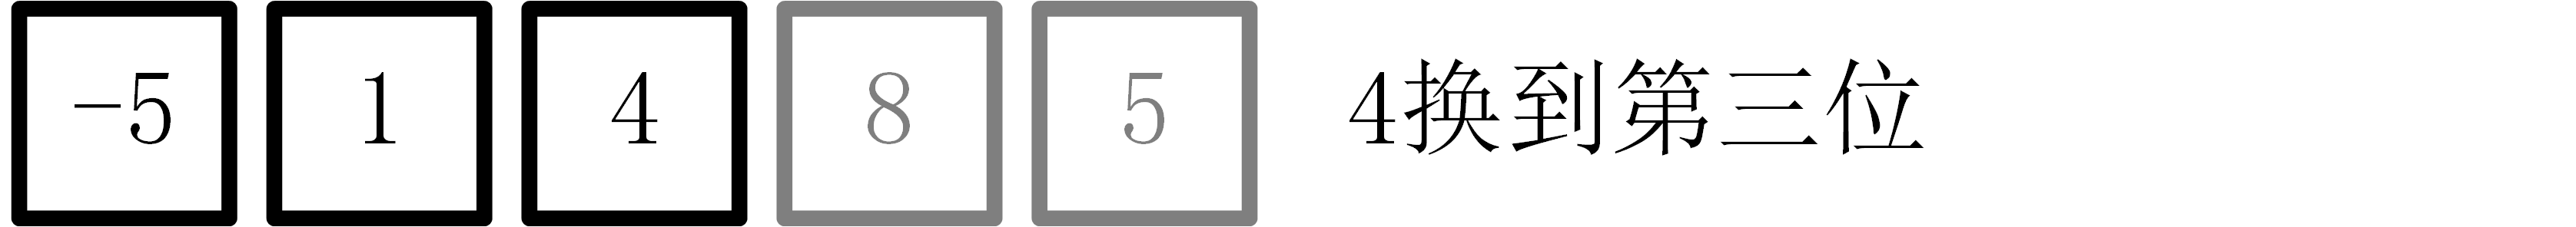
\includegraphics[width=0.8\textwidth]{selection_sort_7}}\\
\uncover<8->{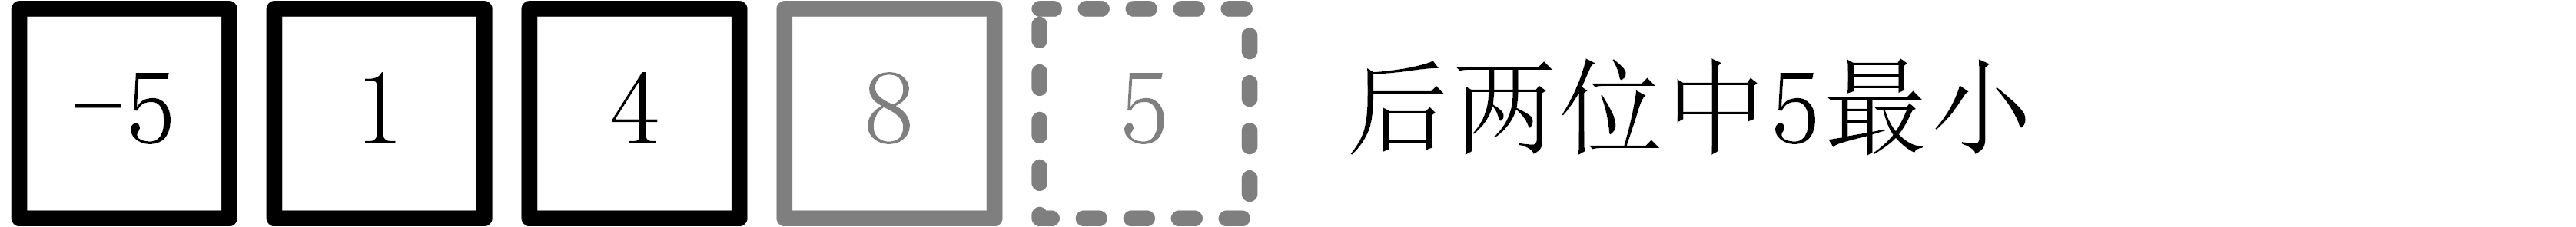
\includegraphics[width=0.8\textwidth]{selection_sort_8}}\\\vspace{-11mm}
\uncover<9->{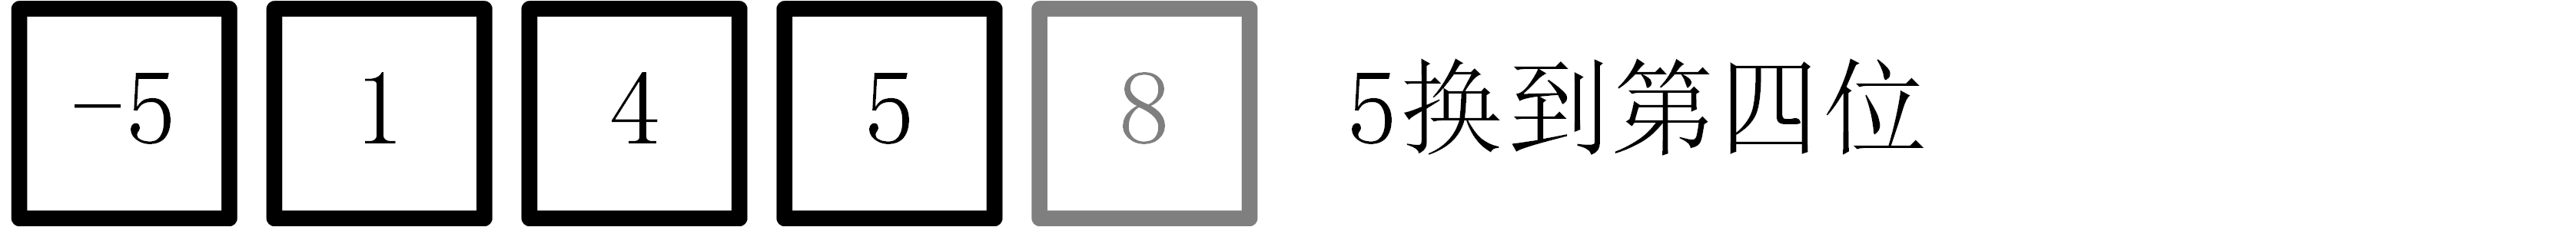
\includegraphics[width=0.8\textwidth]{selection_sort_9}}\\
\uncover<10->{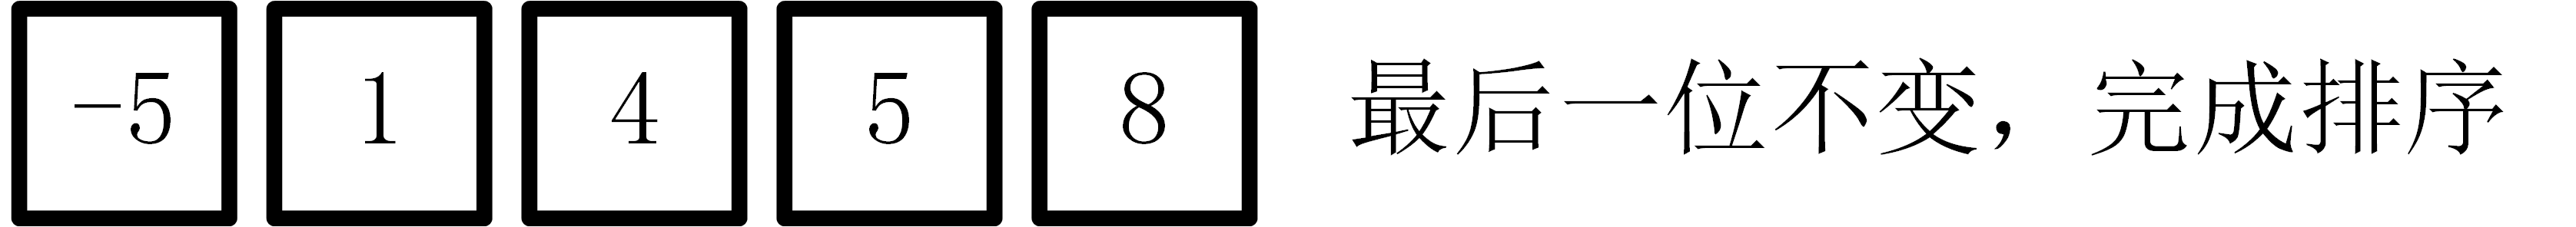
\includegraphics[width=0.8\textwidth]{selection_sort_10}}
\end{center}

\end{frame}

%-----------------

\begin{frame}[fragile]{7.3.1 排序算法\normalsize{~---~选择排序}}

选择排序算法的实现如下:

\vspace{-4mm}

\begin{columns}[t]

\column{0.65\textwidth}
\begin{blueblock}{\texttt{Array}成员函数\texttt{selectionSort}定义}
\begin{lstlisting}[moreemph={Array,T,F}]
template<typename T, size_t N>
template<typename F >
void Array<T, N>::selectionSort(F f) {
    for (int i = 0; i < N - 1; ++i){
        int min = i;        // 记录待排序数据中最小元素位置
        for (int j = i + 1; j < N; ++j) {
            if (f(m_ele[j], m_ele[min]))
                min = j;    //更新最小元素位置
        }
        swap(i, min);       //把最小元素放到位置i
    }
}
\end{lstlisting}
\end{blueblock}

\column{0.3\textwidth}
\begin{yellowblock}{说明}
\texttt{if}语句里的条件表达式将调用函数对象\texttt{f}(\texttt{Less<T>}),检查第一个实参对象是否小于第二个实参对象
\end{yellowblock}

\end{columns}

\end{frame}

%-----------------

\begin{frame}[fragile]{7.3.1 排序算法\normalsize{~---~插入排序}}

将待排序的元素逐个插入已经排好序的元素序列中

\vspace{1mm}

\begin{center}
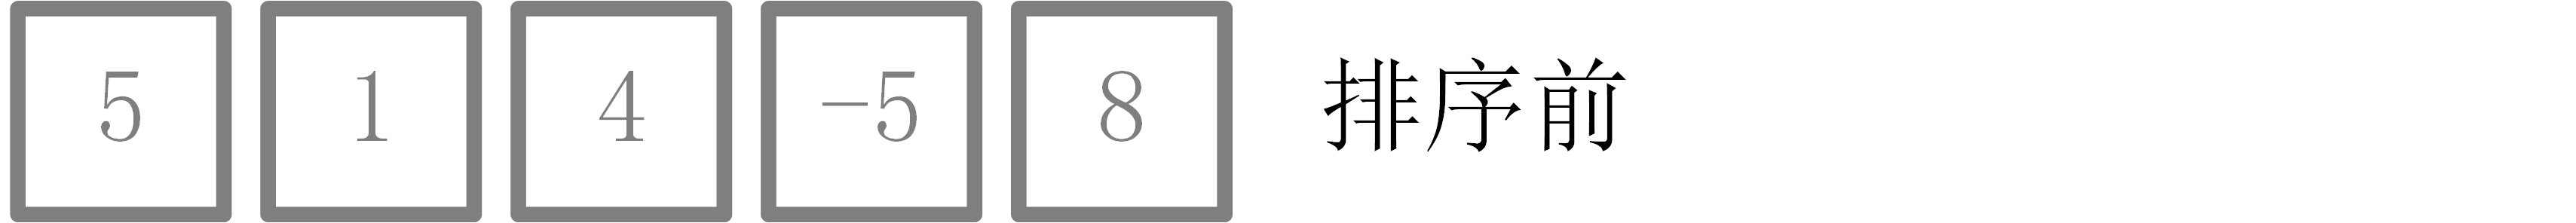
\includegraphics[width=0.8\textwidth]{insertion_sort_1}\\\vspace{3mm}
\uncover<2->{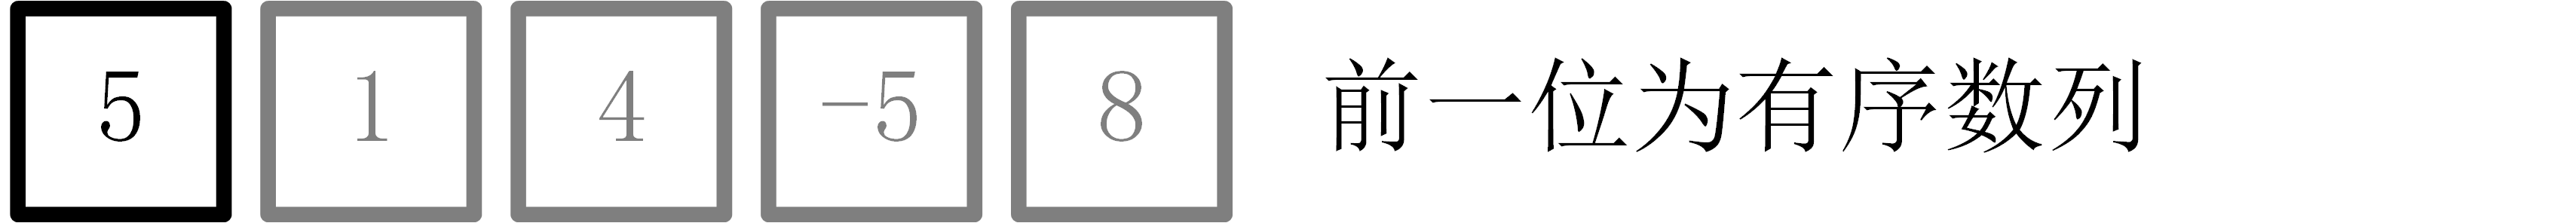
\includegraphics[width=0.8\textwidth]{insertion_sort_2}}\\
\uncover<3->{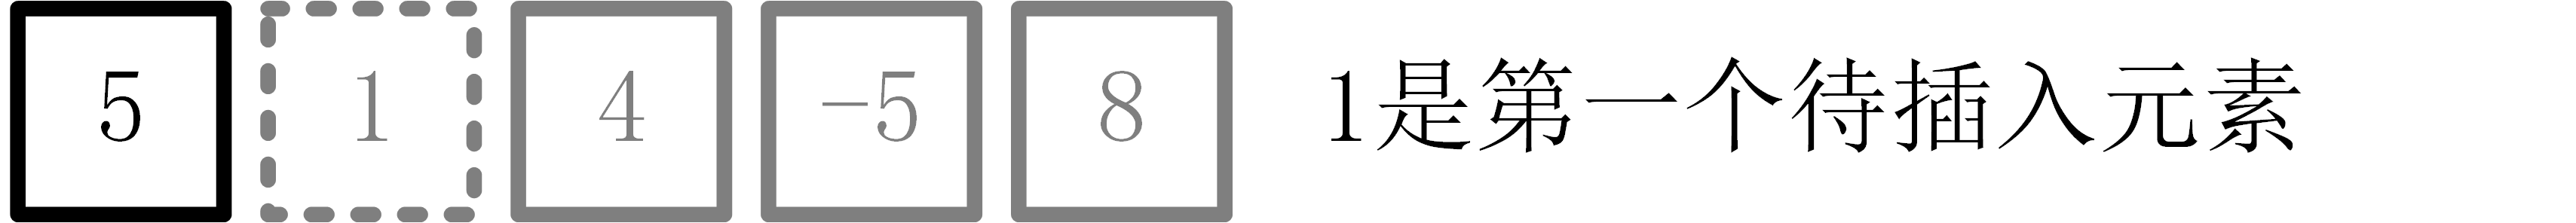
\includegraphics[width=0.8\textwidth]{insertion_sort_3}}\\\vspace{-10.9mm}
\uncover<4->{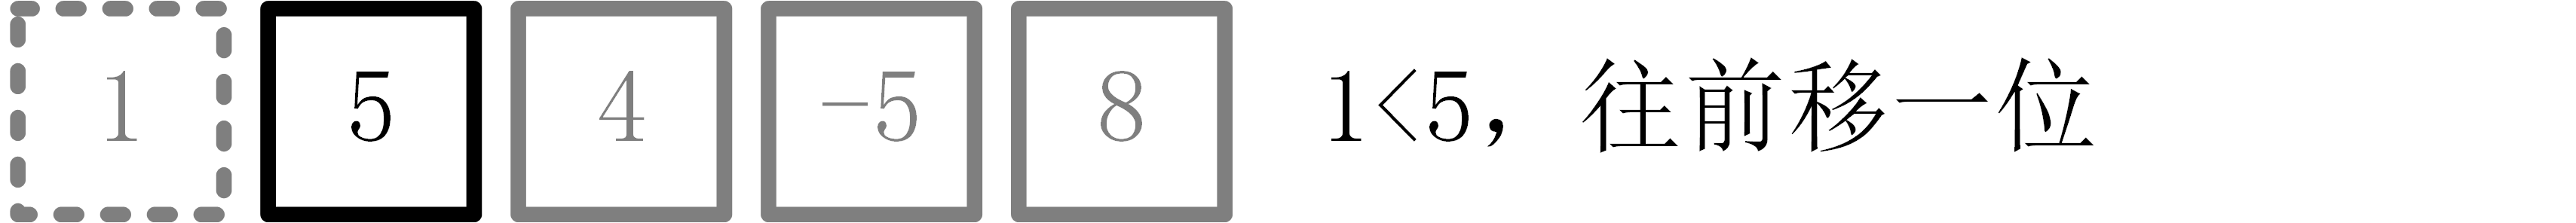
\includegraphics[width=0.8\textwidth]{insertion_sort_4}}\\\vspace{-10.9mm}
\uncover<5->{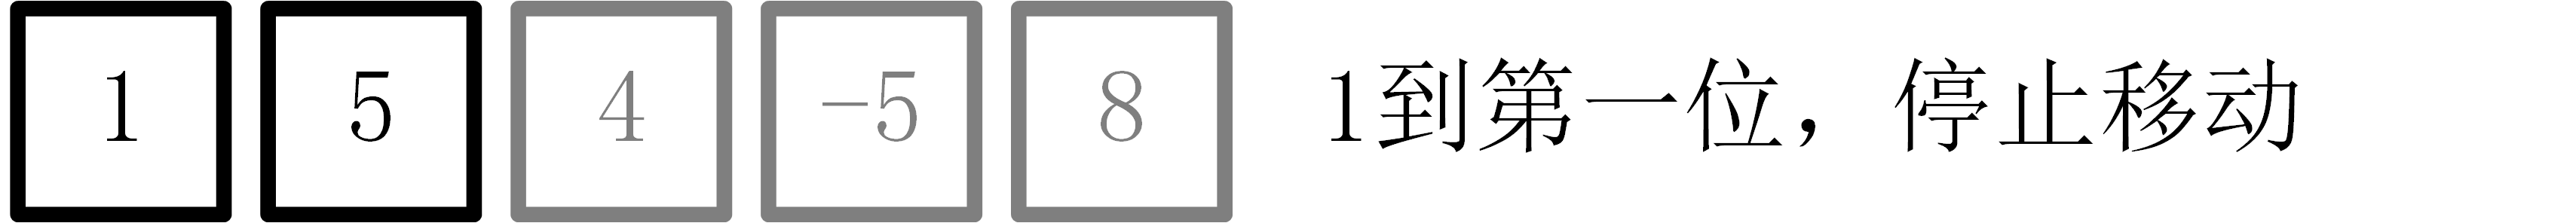
\includegraphics[width=0.8\textwidth]{insertion_sort_5}}\\
\uncover<6->{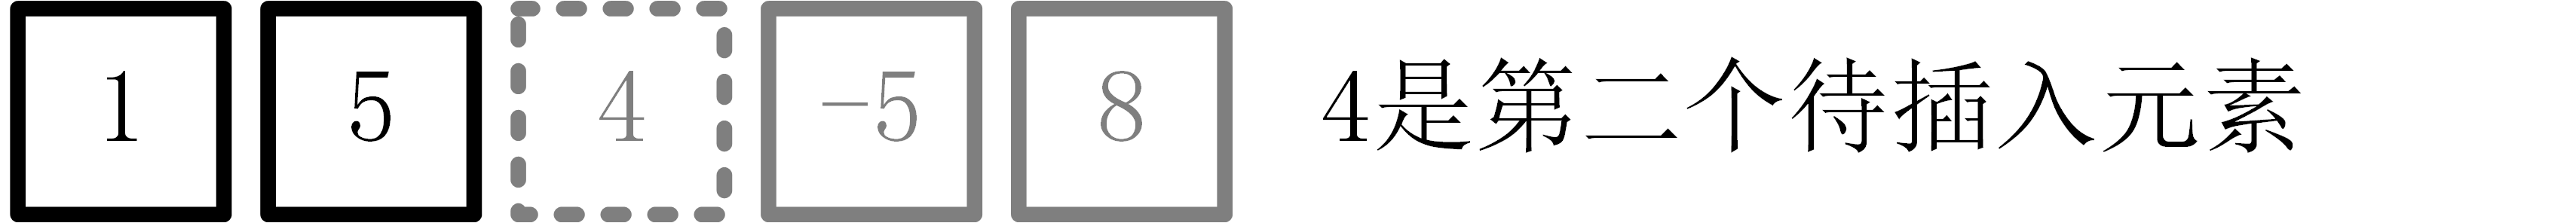
\includegraphics[width=0.8\textwidth]{insertion_sort_6}}\\\vspace{-10.9mm}
\uncover<7->{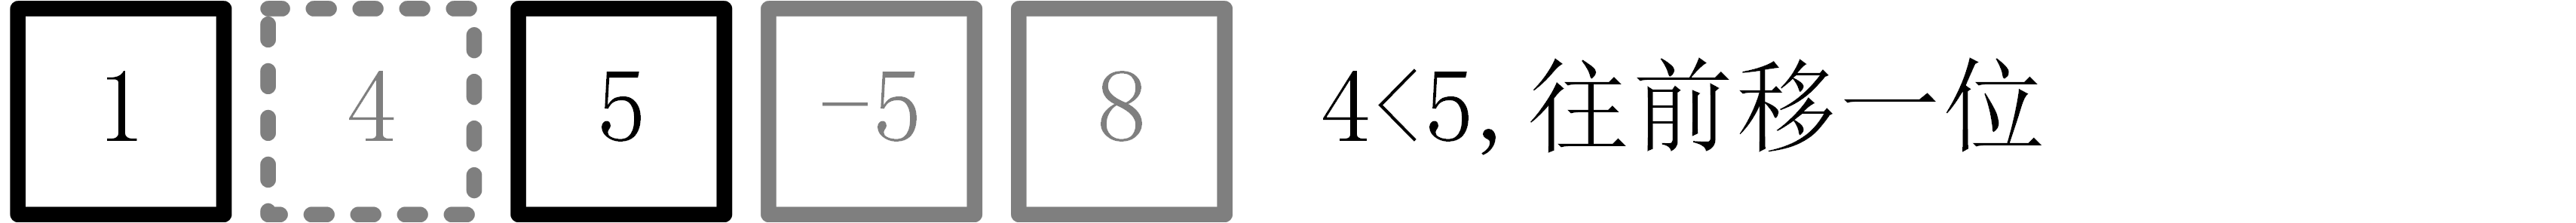
\includegraphics[width=0.8\textwidth]{insertion_sort_7}}\\\vspace{-10.9mm}
\uncover<8->{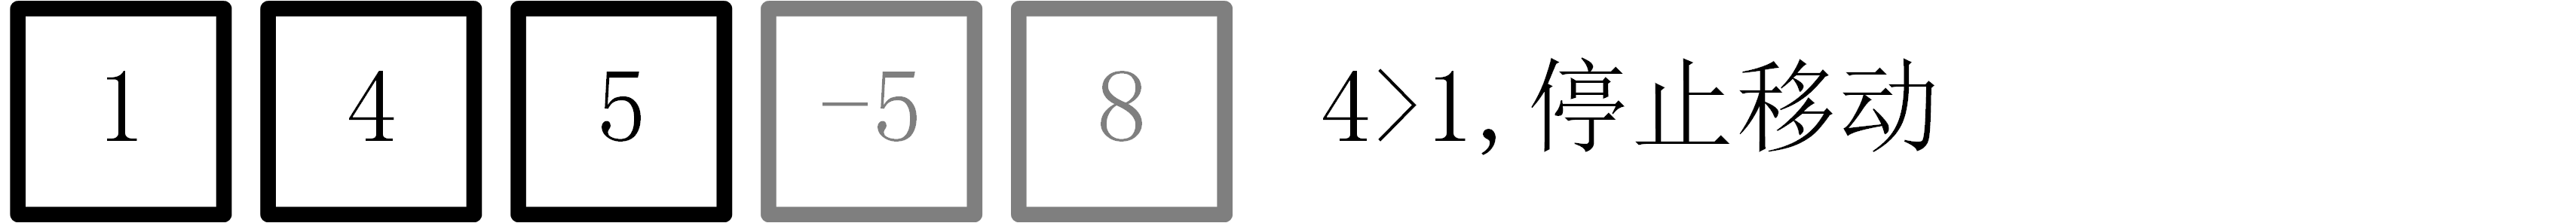
\includegraphics[width=0.8\textwidth]{insertion_sort_8}}\\
\uncover<9->{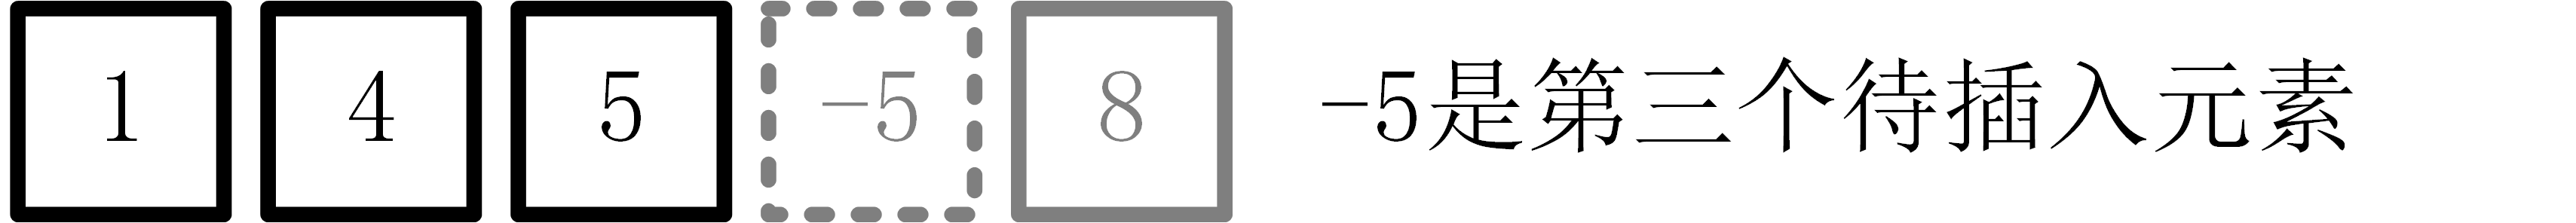
\includegraphics[width=0.8\textwidth]{insertion_sort_9}}\\\vspace{-10.9mm}
\uncover<10->{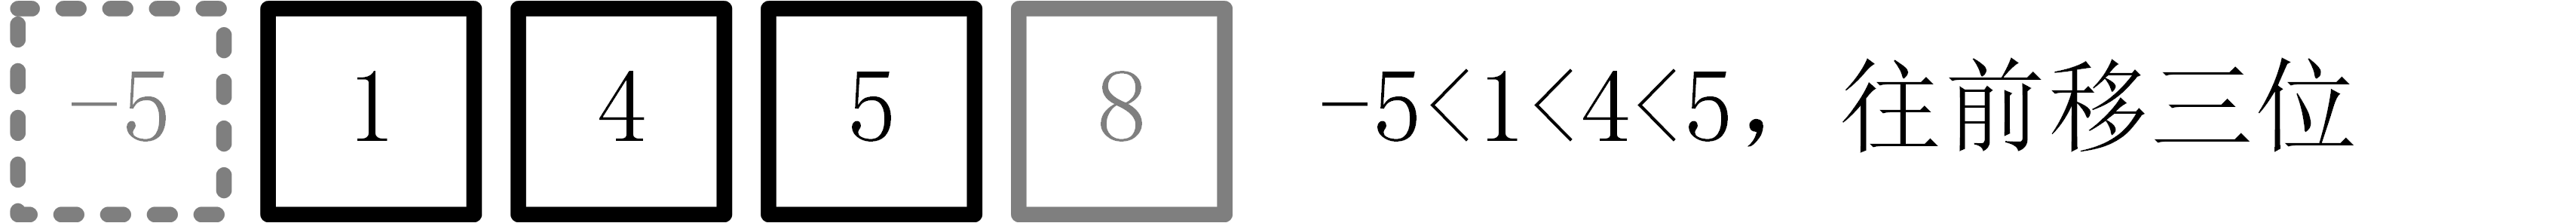
\includegraphics[width=0.8\textwidth]{insertion_sort_10}}\\\vspace{-10.9mm}
\uncover<11->{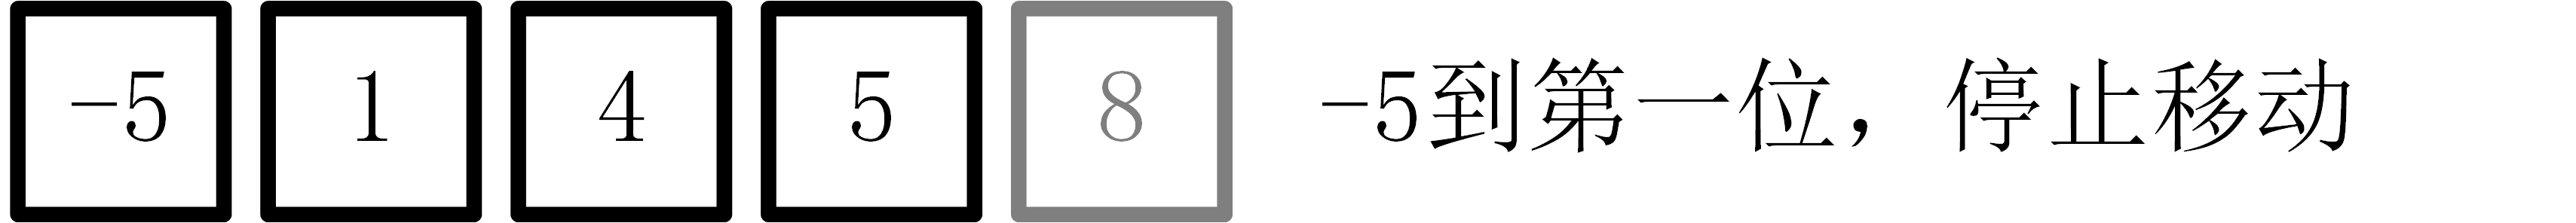
\includegraphics[width=0.8\textwidth]{insertion_sort_11}}\\\vspace{1mm}
\uncover<12->{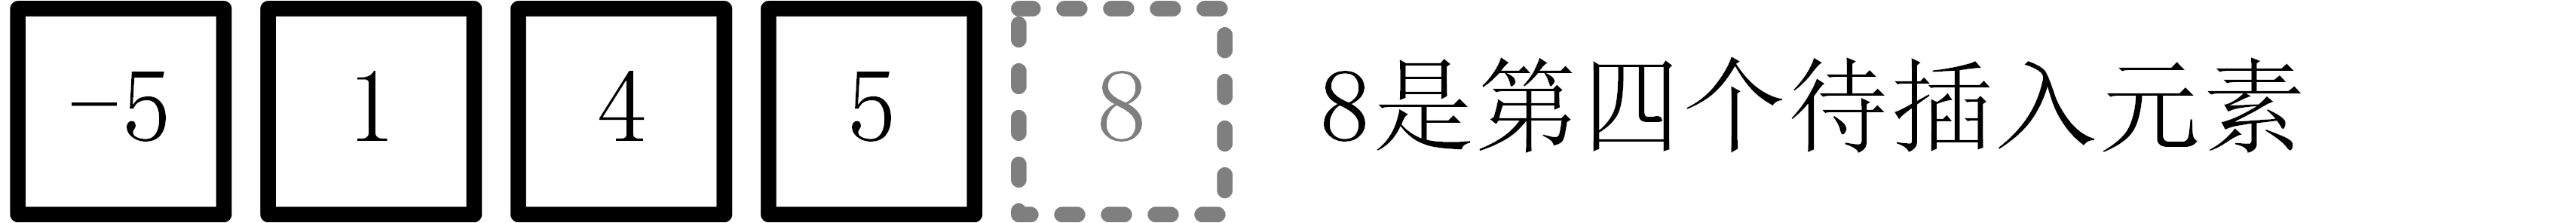
\includegraphics[width=0.8\textwidth]{insertion_sort_12}}\\\vspace{-10.8mm}
\uncover<13->{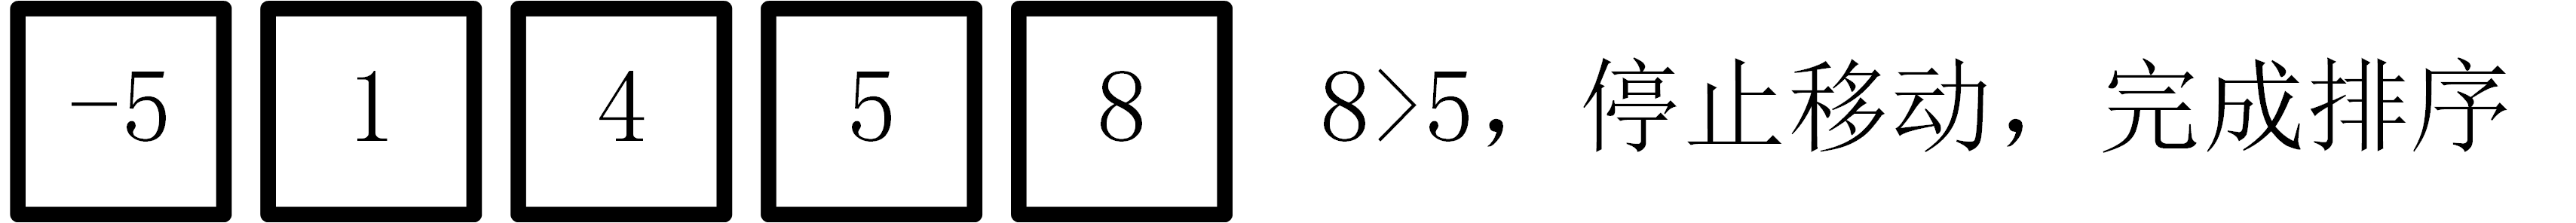
\includegraphics[width=0.8\textwidth]{insertion_sort_13}}
\end{center}

\end{frame}

%-----------------

\begin{frame}[fragile]{7.3.1 排序算法\normalsize{~---~插入排序}}

插入排序算法的实现如下:

\vspace{-4mm}

\begin{columns}[t]

\column{0.65\textwidth}
\begin{blueblock}{\texttt{Array}成员函数\texttt{insertionSort}定义}
\begin{lstlisting}[moreemph={Array,T,F}]
template<typename T, size_t N>
template<typename F >
void Array<T, N>::insertionSort(F f) {
    for (int i = 1, j; i < N; ++i) {
        T t = m_ele[i];                 //待插入元素
        for (j = i; j > 0; --j) {       //查找插入位置
            if (f(m_ele[j - 1], t))
                break;
            m_ele[j] = m_ele[j - 1];    //逐个向后移动元素
        }
        m_ele[j] = t;                   //将待插入元素放到正确位置
    }
}
\end{lstlisting}
\end{blueblock}

\column{0.3\textwidth}

\end{columns}

\end{frame}

%-----------------

\begin{frame}[fragile]{7.3.1 排序算法\normalsize{~---~冒泡排序}}

不断比较相邻的两个元素,如果发现逆序则交换

\vspace{1mm}

\begin{center}
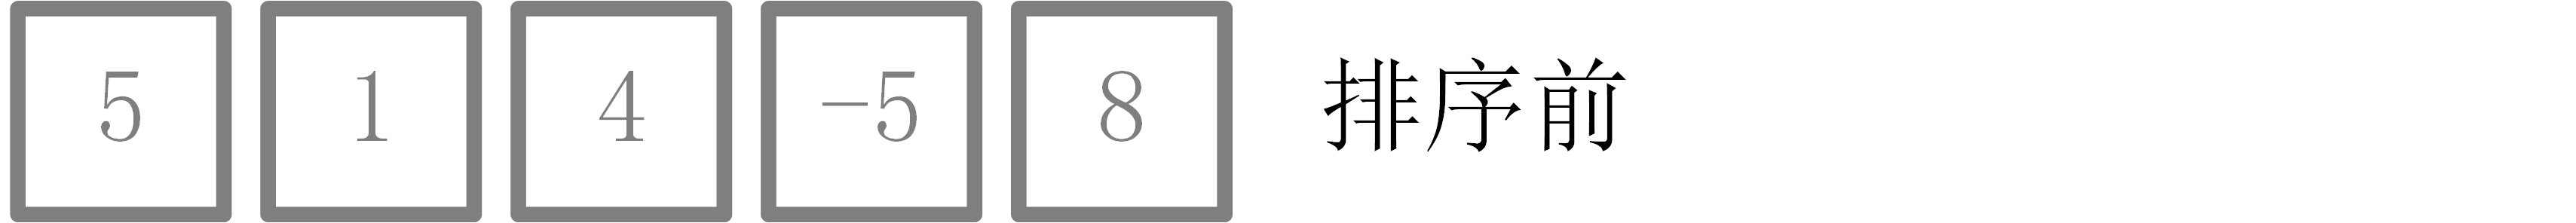
\includegraphics[width=0.8\textwidth]{bubble_sort_1}\\\vspace{3mm}
\uncover<2->{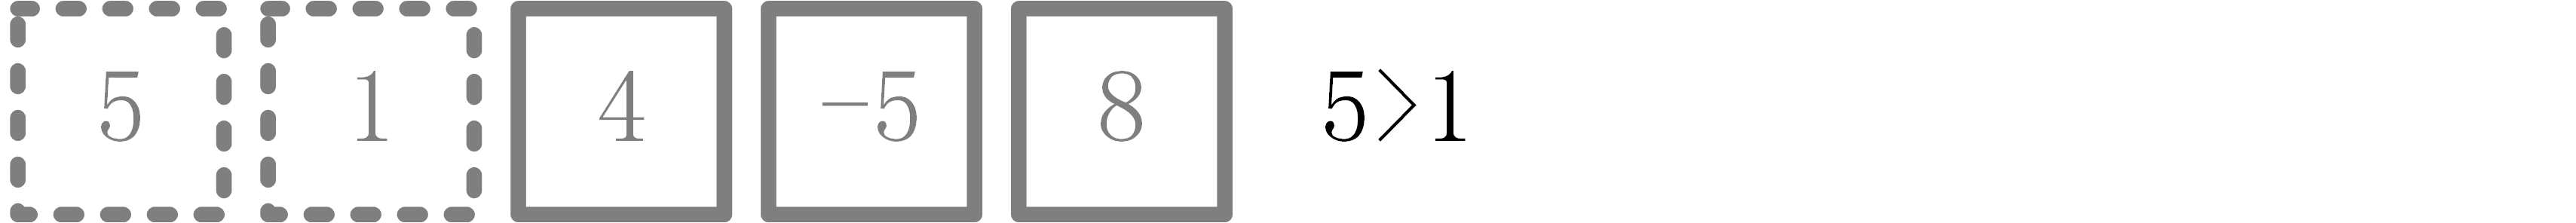
\includegraphics[width=0.8\textwidth]{bubble_sort_2}}\\\vspace{-10.9mm}
\uncover<3->{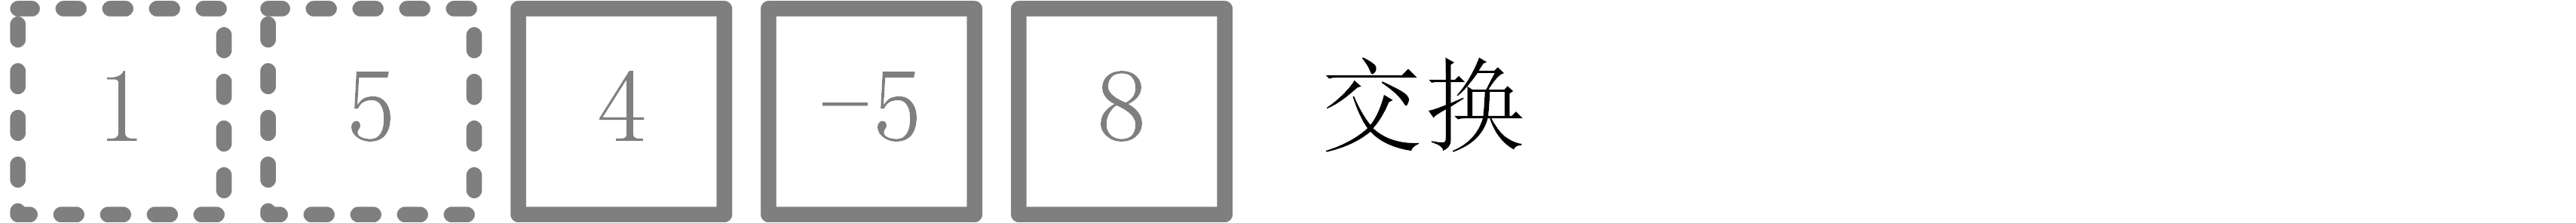
\includegraphics[width=0.8\textwidth]{bubble_sort_3}}\\
\uncover<4->{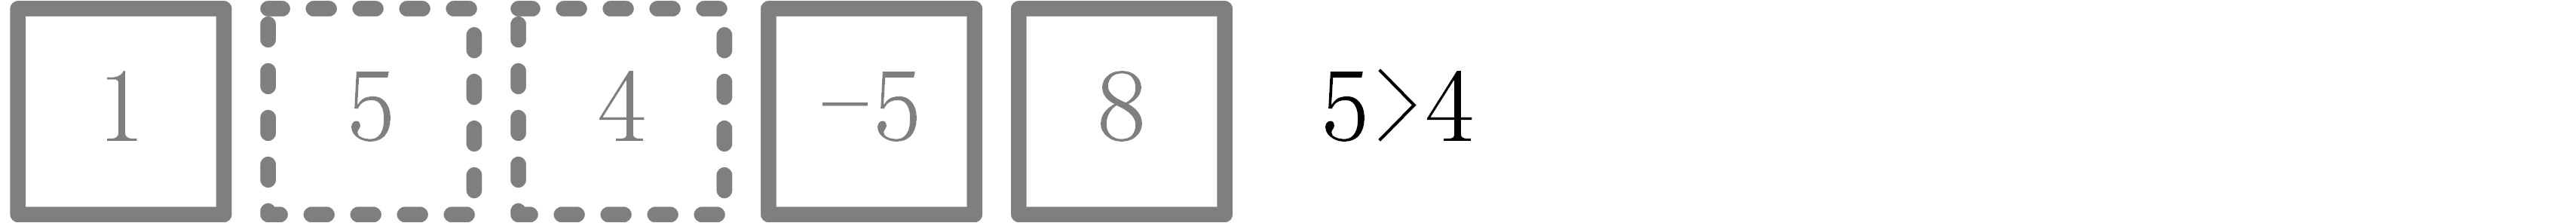
\includegraphics[width=0.8\textwidth]{bubble_sort_4}}\\\vspace{-10.9mm}
\uncover<5->{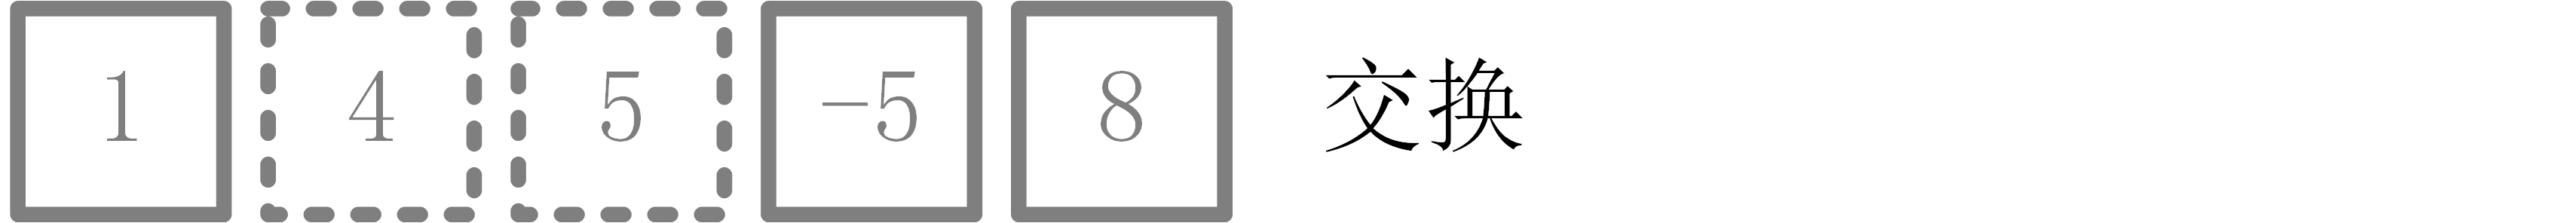
\includegraphics[width=0.8\textwidth]{bubble_sort_5}}\\
\uncover<6->{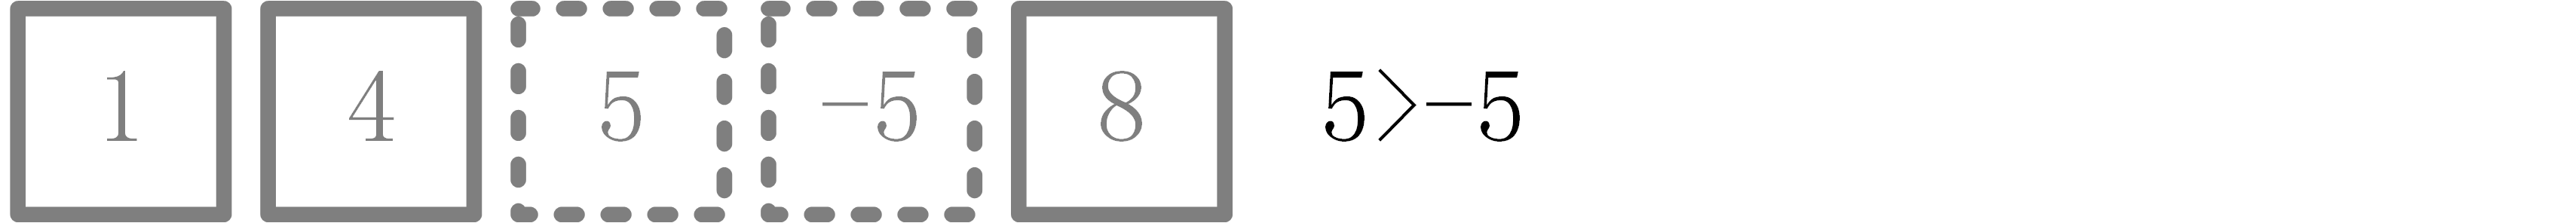
\includegraphics[width=0.8\textwidth]{bubble_sort_6}}\\\vspace{-10.9mm}
\uncover<7->{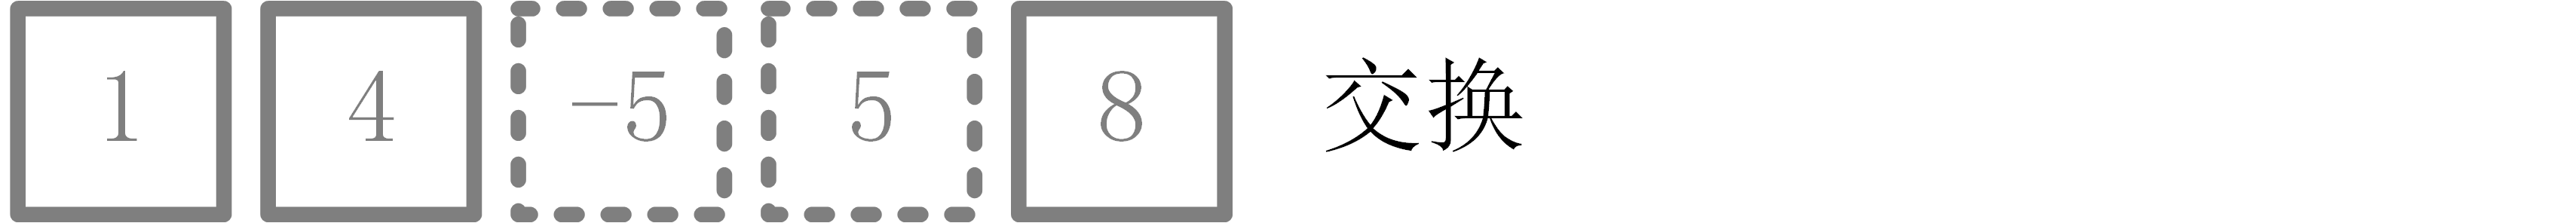
\includegraphics[width=0.8\textwidth]{bubble_sort_7}}\\
\uncover<8->{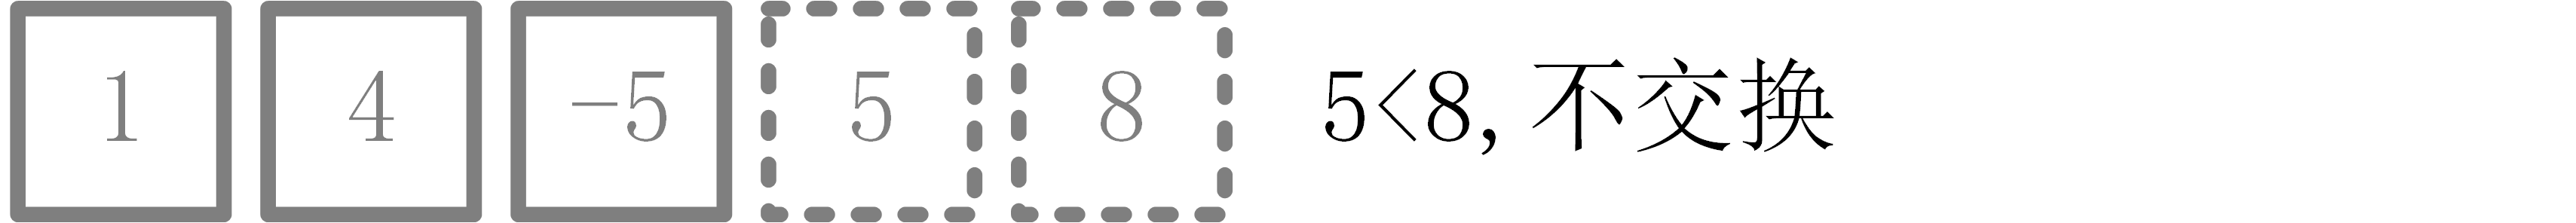
\includegraphics[width=0.8\textwidth]{bubble_sort_8}}\\\vspace{1mm}
\uncover<9->{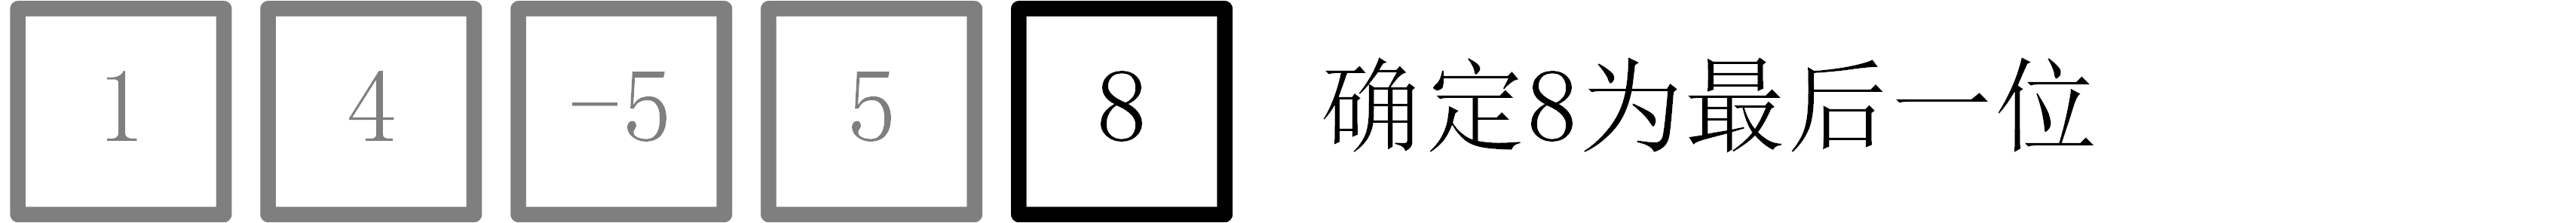
\includegraphics[width=0.8\textwidth]{bubble_sort_9}}
\end{center}

\end{frame}

%-----------------

\begin{frame}[fragile]{7.3.1 排序算法\normalsize{~---~冒泡排序}}

冒泡排序算法的实现如下:

\vspace{-4mm}

\begin{columns}[t]

\column{0.65\textwidth}
\begin{blueblock}{\texttt{Array}成员函数\texttt{selectionSort}定义}
\begin{lstlisting}[moreemph={Array,T,F}]
template<typename T, size_t N>
template<typename F >
void Array<T, N>::bubbleSort(F f){
    for (int i = N - 1; i >= 0; --i){
        for (int j = 0; j <= i - 1; ++j){
            if (f(m_ele[j + 1], m_ele[j]))
                swap(j, j + 1); //相邻元素交换
        }
    }
}
\end{lstlisting}
\end{blueblock}

\column{0.3\textwidth}

\end{columns}

\end{frame}

%-----------------

\begin{frame}[fragile]{7.3.1 排序算法\normalsize{~---~快速排序}}

\begin{block}<1->{快速排序}
 快速排序是冒泡排序的改进,在排序过程中数据移动少。\\
\end{block}
\begin{block}<2->{快速排序的基本思想}
基本思想:划分和分治递归。\\
   \begin{enumerate}
     \item 划分:将整个数组划分为两个部分,第一部分所有值小于基准值(key),第二部分所以值大于基准值(key)。(基准值的选择是随机的,一般选择待排数组的第一个元素)。
     \item 分治递归:第一步将数组划分为两部分后,两部分内部还不是有序的,再分别对两部分递归地进行快速排序,最终得到一个完整的有序数组
   \end{enumerate}
\end{block}
\end{frame}

\begin{frame}[fragile]{7.3.1 快速排序}
快速排序过程

\vspace{1mm}

\begin{center}

\includegraphics[width=0.85\textwidth]{quick_sort1}\\
\uncover<2->{
\includegraphics[width=0.85\textwidth]{quick_sort2}}\\
\uncover<3->{
\includegraphics[width=0.85\textwidth]{quick_sort3}}\\\vspace{-10mm}
\uncover<4->{
\includegraphics[width=0.85\textwidth]{quick_sort4}}\\
\uncover<5->{
\includegraphics[width=0.85\textwidth]{quick_sort5}}\\\vspace{-10mm}
\uncover<6->{
\includegraphics[width=0.85\textwidth]{quick_sort6}}\\
\uncover<7->{
\includegraphics[width=0.85\textwidth]{quick_sort7}}\\
\uncover<8->{
\includegraphics[width=0.85\textwidth]{quick_sort8}}\\\vspace{-10mm}
\uncover<9->{
\includegraphics[width=0.85\textwidth]{quick_sort9}}\\
\end{center}

\end{frame}


%-----------------

\begin{frame}[fragile]{7.3.1 排序算法\normalsize{~---~快速排序}}
\vspace{-2mm}
快速排序算法的实现如下:
\vspace{-1mm}
\begin{blueblock}{}
\vspace{-2mm}
\begin{lstlisting}[moreemph={Array,T,F}]
template<typename T, size_t N>
template<typename F >
void Array<T, N>::quickSort(int left, int right, F f) {
    if (left < right){
        int i = left, j = right;
        T x = m_ele[left];
        while (i < j){
            while (i < j && f(x,m_ele[j]))  j--;    //从右向左找第一个小于x的数
            if (i < j)     m_ele[i++] = m_ele[j];
            while (i < j && f(m_ele[i],x))  i++;    //从左向右找第一个大于等于x的数
            if (i < j)  m_ele[j--] = m_ele[i];
        }
        m_ele[i] = x;
        quickSort(left, i - 1, f);                  //左半部分排序
        quickSort(i + 1, right, f);                 //右半部分排序
    }
}
\end{lstlisting}
\end{blueblock}

\end{frame}
%-------------------------------------
\subsection{二分查找算法}
%-------------------------------------


\begin{frame}[fragile]{7.3.2~二分查找算法}

又称折半查找,在有序序列中使用,其基本思想为分而治之

\vspace{1mm}

\begin{center}
\uncover<2->{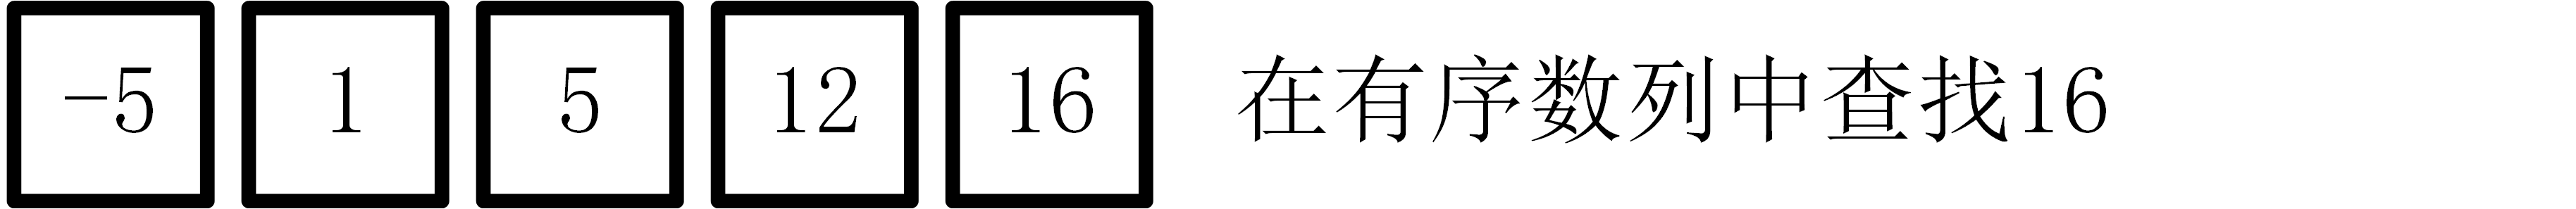
\includegraphics[width=0.8\textwidth]{binary_search_1}}\\\vspace{3mm}
\uncover<3->{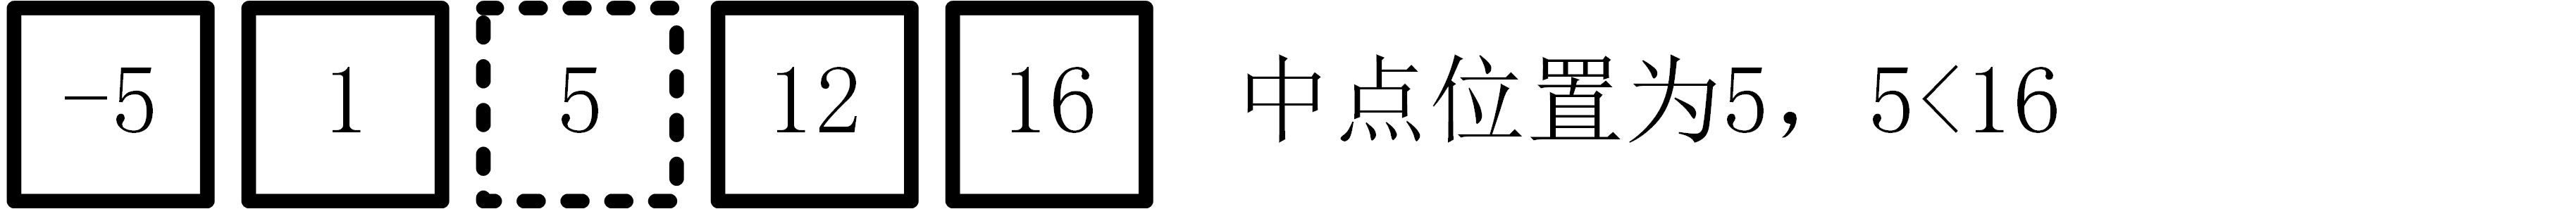
\includegraphics[width=0.8\textwidth]{binary_search_2}}\\\vspace{-10.1mm}
\uncover<4->{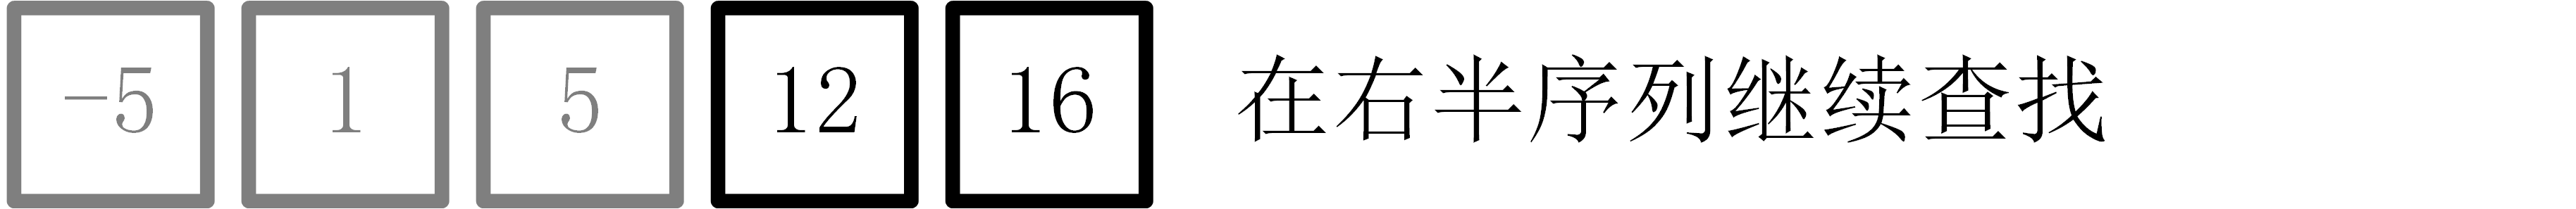
\includegraphics[width=0.8\textwidth]{binary_search_3}}\\\vspace{-10.1mm}
\uncover<5->{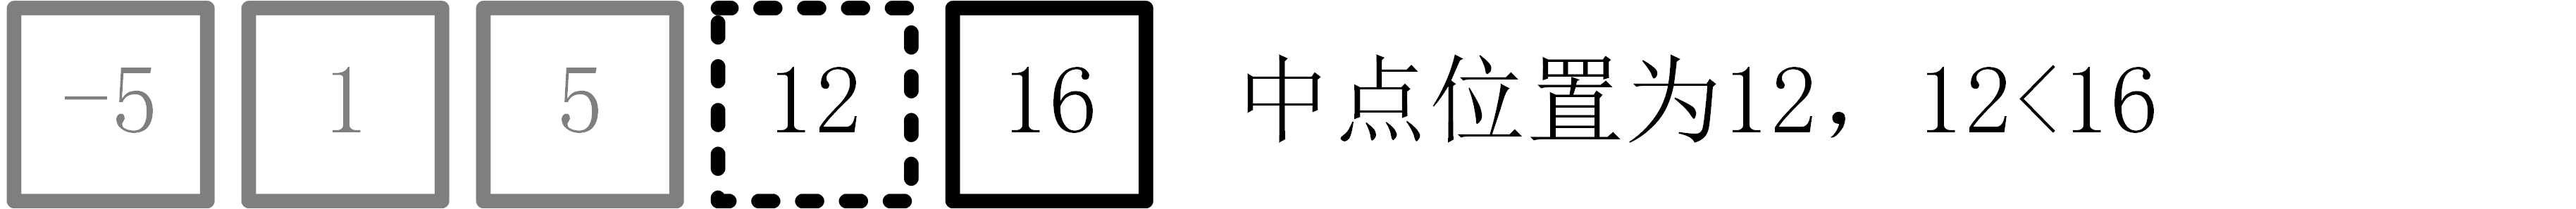
\includegraphics[width=0.8\textwidth]{binary_search_4}}\\\vspace{-10.1mm}
\uncover<6->{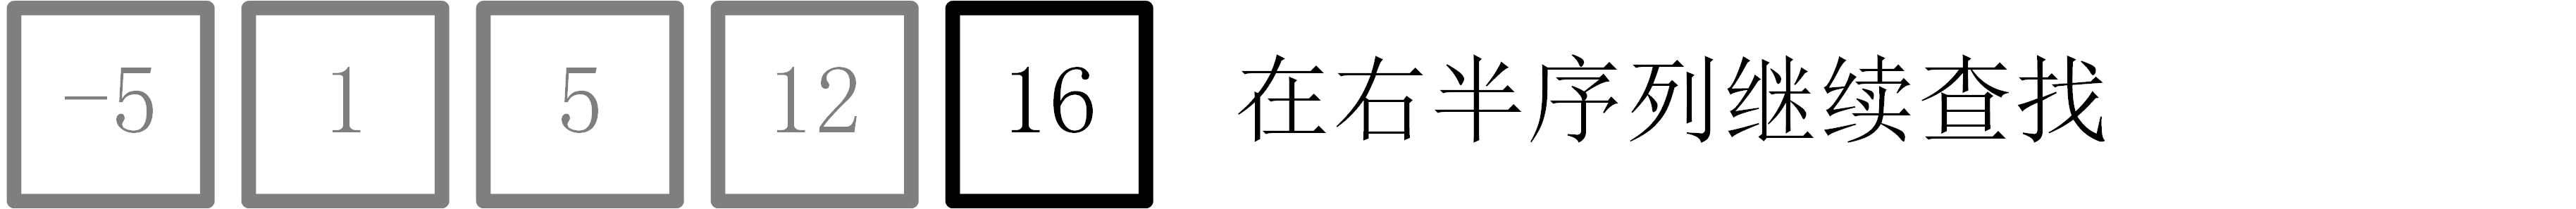
\includegraphics[width=0.8\textwidth]{binary_search_5}}\\\vspace{-10.mm}
\uncover<7->{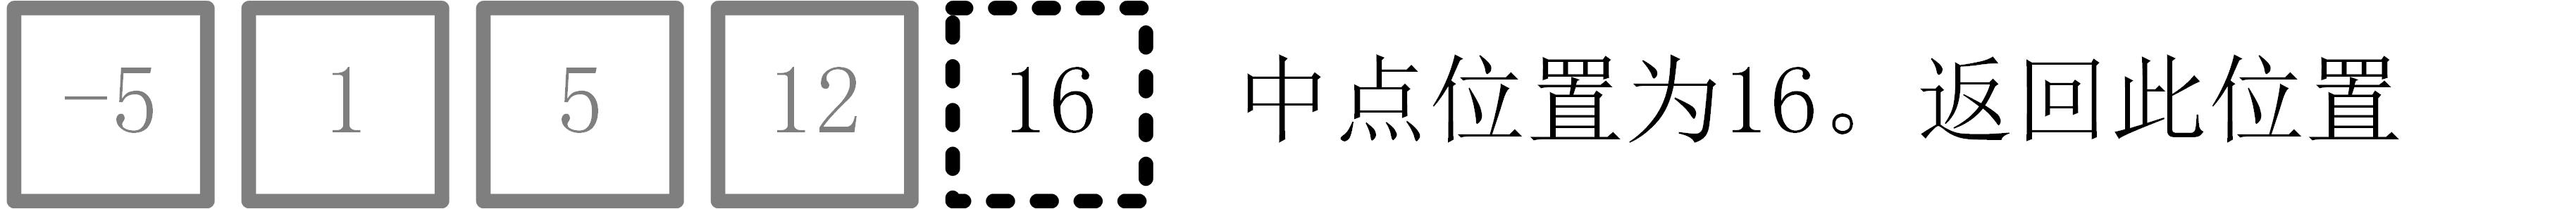
\includegraphics[width=0.8\textwidth]{binary_search_6}}\\\vspace{12mm}
\uncover<8->{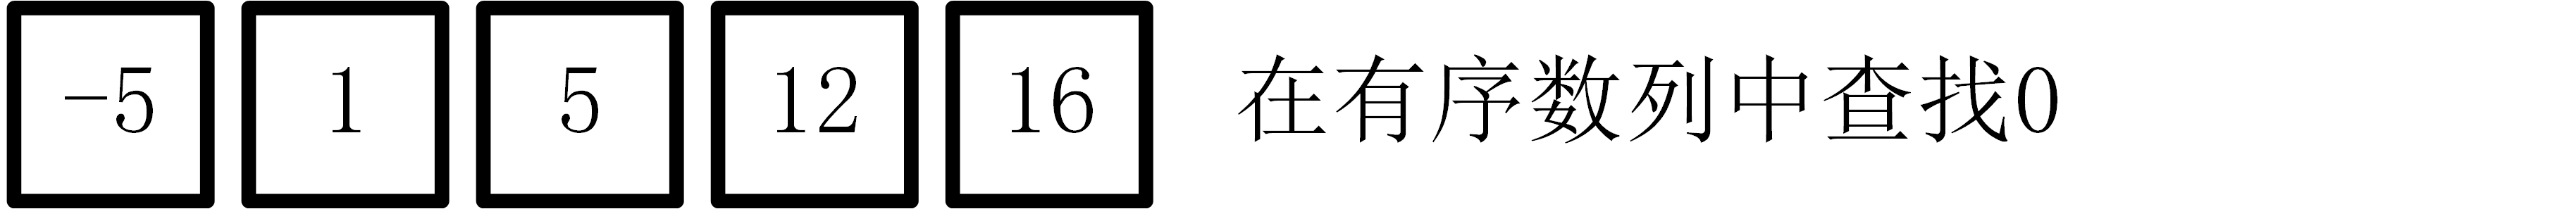
\includegraphics[width=0.8\textwidth]{binary_search_7}}\\\vspace{3mm}
\uncover<9->{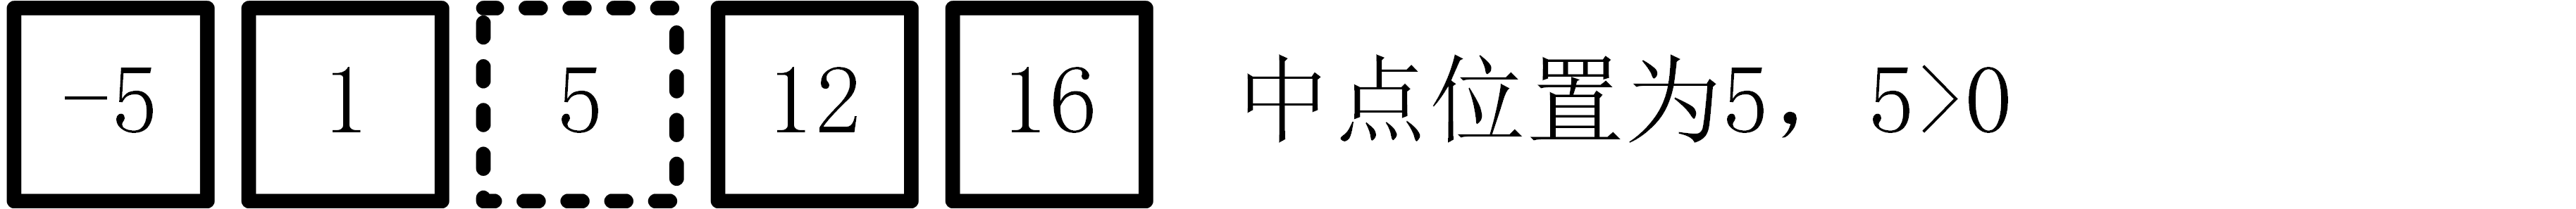
\includegraphics[width=0.8\textwidth]{binary_search_8}}\\\vspace{-10.mm}
\uncover<10->{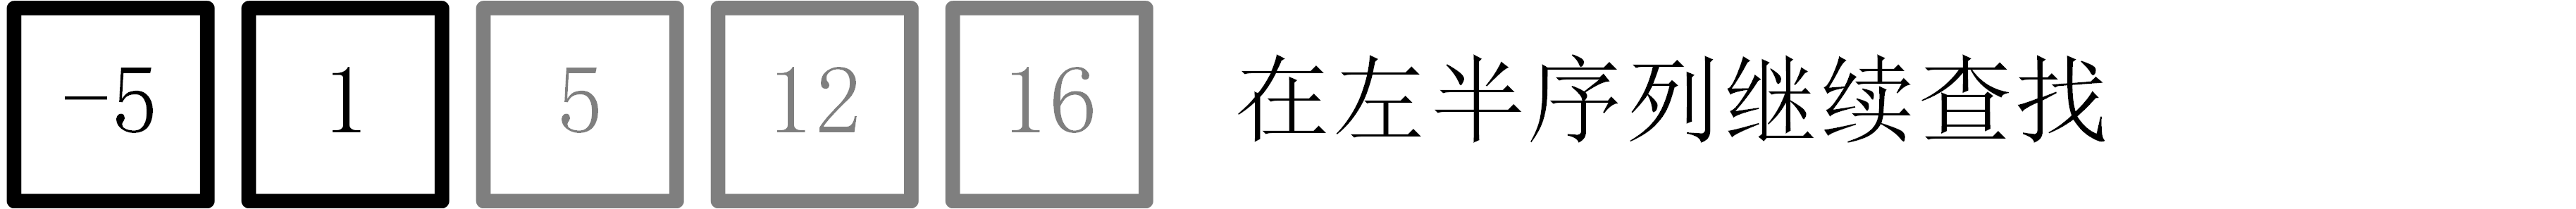
\includegraphics[width=0.8\textwidth]{binary_search_9}}\\\vspace{-10.mm}
\uncover<11->{\includegraphics[width=0.8\textwidth]{binary_search_10}}\\\vspace{-10mm}
\uncover<12->{\includegraphics[width=0.8\textwidth]{binary_search_11}}\\\vspace{-10.mm}
\uncover<13->{\includegraphics[width=0.8\textwidth]{binary_search_12}}\\\vspace{-10.mm}
\uncover<14->{\includegraphics[width=0.8\textwidth]{binary_search_13}}\\\vspace{-10.mm}
\uncover<15->{\includegraphics[width=0.8\textwidth]{binary_search_14}}\\\vspace{-10.mm}
\end{center}

\end{frame}

%-----------------

\begin{frame}[fragile]{7.3.2~二分查找算法}

二分查找算法的实现如下:

\vspace{-4mm}

\begin{columns}[t]

\column{0.65\textwidth}
\begin{blueblock}{\texttt{Array}成员函数\texttt{binarySearch}定义}
\begin{lstlisting}[moreemph={Array,T,F}]
template<typename T, size_t N>
int Array<T, N>::binarySearch(const T &value, int left, int right) {
    while (left <= right) {
        int middle = (left + right) / 2;    //计算中点位置
        if (m_ele[middle] == value)
            return middle;
        else if (m_ele[middle] > value)
            right = middle - 1;             //修改right
        else
            left = middle + 1;              //修改left
    }
    return -1;                              //查找失败
}
\end{lstlisting}
\end{blueblock}


\column{0.3\textwidth}
\begin{yellowblock}{说明}
$\bullet$ \texttt{value}小于中点位置元素,将\texttt{right}设为\texttt{middle-1}\\
$\bullet$ \texttt{value}大于中点位置元素,将\texttt{left}设为\texttt{middle+1}\\
$\bullet$ 查找失败则返回\texttt{-1}
\end{yellowblock}
\vspace{-2mm}
\begin{greenblock}<2->{问题}
查找\texttt{4}返回时,\texttt{left}和\texttt{right}的值是多少?
\end{greenblock}
\vspace{-2mm}
\begin{greenblock}<3->{答案}
\texttt{left}为\texttt{2},\texttt{right}为\texttt{1}
\end{greenblock}

\end{columns}

\end{frame}

%-----------------

\begin{frame}[fragile]{7.3.2~改进插入排序算法效率}

\begin{greenblock}{问题}
如何改进插入排序算法的效率?
\end{greenblock}

\end{frame}
